% Chapter 3 - Methodology
% With Sample Figures From Kevin Hughes

\glsresetall % reset the glossary to expand acronyms again
\chapter[Methodology]{Methodology}\label{ch:Methodology}
\index{Methodology}


This chapter provides a detailed breakdown of the research procedures undertaken to compare the suitability of two deep learning models, \gls{N2N} and \gls{N2V} as potential denoising models for the  LODOX\textsuperscript{\textregistered} Statscan\textsuperscript{\textregistered}. It begins with an in-depth analysis of the user and functional requirements, followed by a detailed analysis of the research design. Theoretical background and analysis of \gls{N2N} and \gls{N2V} models are then addressed, after which an exploration of the various research instruments used to develop them, ranging from software to hardware tools is addressed. Data collection is then explored in detail, exploring the various phantoms used and the rationale behind their use. This is followed by analysing the performance evaluation metrics to evaluate the two models. The chapter culminates with an analysis of the limitations and ethical concerns associated with the study. 

\section{Model Development and Comparison Procedure}
The methodology followed the waterfall approach and is broken down into the following phases and summarised in Figure \ref{fig:method} below:

\begin{enumerate}
    \item {\textbf{Literature Review and Familiarisation:} This phase involved an extensive review of existing medical imaging denoising techniques and learning the tools and technologies essential for the project. This included understanding the operational principles of the LODOX\textsuperscript{\textregistered} Statscan\textsuperscript{\textregistered} system, gaining familiarity with \gls{PCD} technology, and working with programming languages commonly used in denoising models, such as Python and MATLAB\textsuperscript{\textregistered}.}

    \item \textbf{Data Collection and Pre-Processing:} This phase involved configuring the LODOX\textsuperscript{\textregistered} Statscan\textsuperscript{\textregistered} with the required parameters and scanning the selected phantoms. After scanning the phantoms, the images were exported through DVS\textsuperscript{\textregistered} software for pre-processing, which included normalisation, data type conversion, and the addition of extra dimensions.
    \item \textbf{Model Selection and Design:} This phase involved developing and implementing the suitable models identified in Phase 1, specifically \gls{N2V} and \gls{N2N}, due to their adaptability and ability to train without clean images. Variations of these models were implemented in Python programming language on the Google Colab cloud platform.
    \item \textbf{Model Training and Validation:} The data set was split into a training(80\%) set and a validation(20\%) set. The models were trained in two stages. The first stage involved using ten training images over 50 epochs with 100 training steps per epoch. The second stage involved 29 images over 150 epochs with 100 training steps per epoch. After each phase, the training and validation loss and \gls{MSE} were analysed to evaluate model generalisation, with hyperparameter tuning performed as needed.
    \item \textbf{Model testing and evaluation: }In this phase, a new test set of 10 images not used in training was collected. These images were passed through the models, and performance metrics such as proxy \gls{SNR}, \gls{PSNR}, and \gls{SSIM} were calculated to assess the models' suitability for the LODOX\textsuperscript{\textregistered} Statscan\textsuperscript{\textregistered} system.
    \item \textbf{\gls{GUI} Development:} Once the model was tested and the results analysed, a \gls{GUI} was created to enable easy denoising of the images using the two models. This \gls{GUI} is a preliminary step for further integrating the denoising models into the LODOX\textsuperscript{\textregistered} DVS\textsuperscript{\textregistered} Software.
\end{enumerate}

 \begin{figure}[h!]
     \centering
     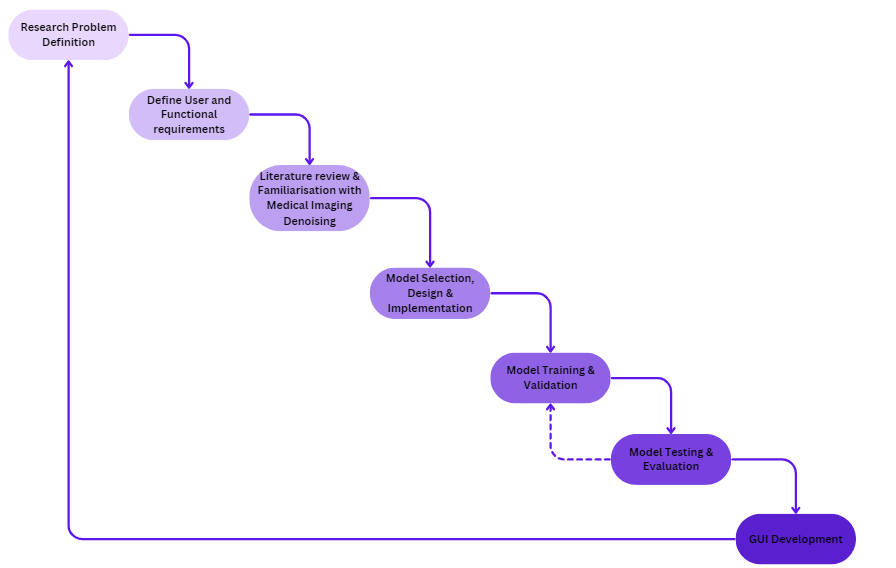
\includegraphics[width=0.9\linewidth]{3_Chapters//3_Chapter_Methodology//Figures/Waterfall.png}
     \caption{Waterfall models depicting the methodology overview}
     \label{fig:method}
 \end{figure}

 \section{System Requirements} \label{sec:reqs}
 The user requirements for the system are detailed in Table \ref{tab:UR} below:

 \begin{table}[h!] 
    \small
    \centering
    \caption{User Requirements} 
    \label{tab:UR} 
    \begin{tabular}{@{}llp{7cm}@{}} 
    \toprule 
    \textbf{ID }& \textbf{Requirement} &\textbf{Description} \\ 
    \midrule 
    UR-01 & High Image Quality & The model should significantly enhance the clarity and quality of LODOX\textsuperscript{\textregistered} Statscan\textsuperscript{\textregistered} images. \\ 
    UR-02 & Retention of Anatomical Details & The model should preserve critical anatomical structures within the images. \\ 
    UR-03 & Compatibility with Existing Systems & The model should be compatible with existing medical imaging software and systems. \\ 
    UR-04 & Fast Processing Time & The model should process images quickly to support real-time diagnostic workflows. \\ 
    UR-05 & User-Friendly Interface & The model should provide an intuitive interface to apply the denoising model easily. \\ 
    UR-06 & Scalability & The model should handle varying image sizes and resolutions effectively. \\ 
    UR-07 & Robustness Across Noise Levels & The model should effectively reduce noise in images with varying noise intensity levels. \\ 
    UR-08 & Minimal Artifact Introduction & The model should minimise the introduction of artifacts during the denoising process. \\ 
    \bottomrule 
    \end{tabular} 
    \end{table}

    These user requirements are then used to derive the functional requirements of the system which are then  detailed in the Table \ref{tab:FR} below:
    \begin{table}[h!]
        \small
        \centering
        \caption{System Functional Requirements}
        \label{tab:FR}
        \begin{tabular}{@{}lp{3cm}p{5cm}p{4cm}@{}}
        \toprule
        \textbf{ID} &
          \textbf{Requirement} &
          \textbf{Description} &
          \textbf{User Requirement} \\ \midrule
        FR-01 &
          Image Quality Enhancement &
          The model shall enhance SNR and PSNR to improve overall image clarity. &
          UR-01 \\
        FR-02 &
          Anatomical Detail Preservation &
          The model shall optimise \gls{SSIM} to ensure critical anatomical structures are preserved. &
          UR-02 \\
        FR-03 &
          System Compatibility &
          The model shall integrate with \gls{DICOM}-compliant medical imaging software, such as DVS\textsuperscript{\textregistered} by LODOX\textsuperscript{\textregistered}. &
          UR-03 \\
        FR-04 &
          Efficient Processing &
          The model shall denoise a standard LODOX\textsuperscript{\textregistered} Statscan\textsuperscript{\textregistered} image within 5 seconds. &
          UR-04 \\
        FR-05 & User Interface Design  & The model shall provide a \gls{GUI} for uploading, processing, and downloading images with minimal steps.          & UR-05 \\
        FR-06 & Scalability Features   & The model shall support various input image resolutions and dimensions, adjusting algorithms accordingly.    & UR-06 \\
        FR-07 & Noise Level Adaptation & The model shall adaptively filter images with different noise levels to maintain high-quality output.        & UR-07 \\
        FR-08 & Artifact Minimisation  & The model shall include techniques to detect and minimise artifacts introduced during the denoising process. & UR-08 \\ \bottomrule
        \end{tabular}
        \end{table}

\section{Research Design}
\subsection{Familiarisation With Medical Imaging Denoising Techniques}
Relevant literature detailing the various algorithms used in X-ray image denoising was explored, with a particular focus on methods that are effective in denoising photon-limited images with Poisson noise as the LODOX\textsuperscript{\textregistered} Statscan\textsuperscript{\textregistered} images meet that criterion. Deep learning methods were given precedence as they are adaptable across various noise types and outperform most classical filters when trained sufficiently. In exploring the deep learning denoising models focus was on unsupervised models i.e that do not require clean images for denoising. This was covered in detail in Chapter \ref{ch:LitReview}. 

\subsection{Preliminary Data Collection}
Preliminary data was collected to familiarise ourselves with the LODOX\textsuperscript{\textregistered} Statscan\textsuperscript{\textregistered} system, given it was our first time working with the scanner. Additionally, this data helped in selecting appropriate phantoms to be used to train the ML models. This was through evaluating the performance of classical filters namely \gls{NLM},\gls{BM3D} and Wavelet at default settings on the data using \gls{SNR} and \gls{PSNR}.  Phantom images that most of the classical filters struggled to denoise were then selected to be used for training. This ensured that only noise-rich phantom images could be used to train the Deep-learning models.

\subsection{Model Selection and Preliminary Testing}
\label{sec:modsec}
Two critical factors guided the selection of the models to be used, i.e adaptability to learn to denoise across various noise types and not requiring clean images to learn denoising. Additionally, previous tests or applications of the models on medical image denoising or photon-limited image settings such as microscopy images was considered. The two models that met that criteria were \gls{N2N} and \gls{N2V}. They both use noisy image inputs to learn the denoising as was detailed in \ref{sec:deeplearning}. Moreover, \gls{N2N} had previously been tested on denoising \gls{MRI}. Although \gls{MRI} is predominantly affected by Rician noise, \gls{N2N} is highly adaptable and can learn to denoise photon-limited images with sufficient training. In contrast, \gls{N2V} was predominantly tested on microscopy images that are degraded by Poisson noise. Although, this is not the same condition as in LODOX\textsuperscript{\textregistered} Statscan\textsuperscript{\textregistered}
 given the high levels of Poisson noise, \gls{N2V} is highly adaptable and has the potential to effectively denoise LODOX\textsuperscript{\textregistered} Statscan\textsuperscript{\textregistered}
images. 

These two models were then assessed using the preliminary data collected to understand how they perform and how various parameters can be adjusted further to enhance their performance on the LODOX\textsuperscript{\textregistered} Statscan\textsuperscript{\textregistered}
images. This involved training them for 10 epochs with 10 iterations per epoch using only a single image for \gls{N2V} and two images for \gls{N2N}. 

\subsection{Data Collection} \label{sec:datacolelction}
\textbf{Phantom Types} \label{sec:phantom} \\
Primarily, two classes of phantoms were used in this study, as discussed below:
\begin{enumerate}
    \item \textbf{Medical Calibration Phantoms: } Used for \gls{CT} scans and bone density measurements. These phantoms are the clsest to human anatomy and are used to calibrate the LODOX\textsuperscript{\textregistered} Statscan\textsuperscript{\textregistered} system.
    \item \textbf{Everyday Objects:}  Include keyboards, calculators, metallic rulers, glass funnels, etc., used to model various noise scenarios and provide noise-rich images for model training.
\end{enumerate}

\textbf{Phantom Selection Criteria} \\
The following criteria were used in selecting phantoms for scans:
\begin{enumerate}
    \item \textbf{Affordability and availability:} only phantoms that were freely available to my supervisor and those provided by LODOX\textsuperscript{\textregistered} were used. This meant that anatomical phantoms were not available.
    \item \textbf{Artifacts Generation: }phantoms that were highly known to introduce artfiacts were used to deliberately introduce artifacts in the images so that the model could learn to remove such from the images.
    \item \textbf{Presence of edges:} since most denoising models struggle with preserving edges, phantoms with nice and straight edges were also incorporated to aid in model training and test the trained model's ability to preserve edges, as this is a critical part of denoising.
\end{enumerate}

\textbf{Data Collection Procedure} \\
Informed from findings from \ref{sec:phantom}, new phantom scans of the noise-rich objects were scanned. This included the following phantoms scanned from various angles:

\begin{enumerate}
    \item A Variety of tools available at the lab
    \item Level
    \item Keyboard
    \item Computer Mouse
    \item Calculator
    \item Smartphone
\end{enumerate}

The following scanning conditions were employed:

\begin{enumerate}
    \item The scanning was done strictly during the day
    \item The following parameters were set on the LODOX\textsuperscript{\textregistered} Statscan\textsuperscript{\textregistered} scanner for the scanning as detailed in Table \ref{tab:scansettings} below:
\end{enumerate}

\begin{table}[h!]
    \centering
    \caption{LODOX\textsuperscript{\textregistered} Statscan\textsuperscript{\textregistered} scanner configuration}
    \label{tab:scansettings}
    \begin{tabular}{@{}ll@{}}
    \toprule
    \textbf{Metric/Parameter} & \textbf{Setting Used} \\ \midrule
    Procedure                 & Chest(lung) AP        \\
    Scan Time                 & 0.00 ms               \\
    Exposure Time             & 66.00 ms              \\
    X-ray tube current        & 50.00 mA              \\
    X-ray Tube Voltage        & 120 kV(KVP)           \\
    Detector Binning          & 2                     \\
    Scan Velocity             & 140 mm/s              \\
    Spatial Resolution        & 5.00 lp/mm            \\ \bottomrule
    \end{tabular}
\end{table}


After the scans, all the processing done by the DVS\textsuperscript{\textregistered} software by LODOX\textsuperscript{\textregistered} was removed by unchecking the Lucid(R) and Denoise filters applied in the processing history menu, as shown in Figure \ref{fig:menu} below. This ensured raw, unprocessed images were exported for model training. 

\begin{figure}[h!]
    \centering
    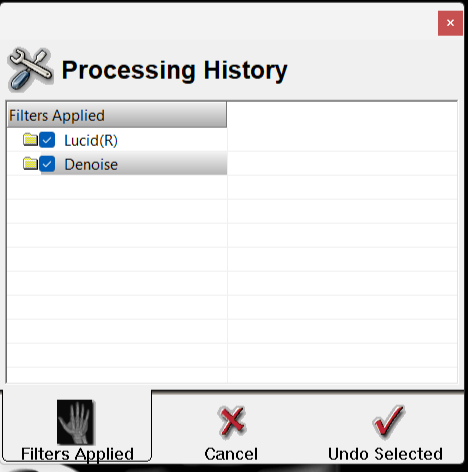
\includegraphics[width=0.64\linewidth]{3_Chapters//3_Chapter_Methodology//Figures/Filteruncheck.png}
    \caption{Illustration of unchecking the custom filters in the DVS\textsuperscript{\textregistered} processing history menu}
    \label{fig:menu}
\end{figure}

A total of 10 images were collected for training as shown in Figure \ref{fig:trainingset} below:
\begin{figure}[h!]
    \centering
    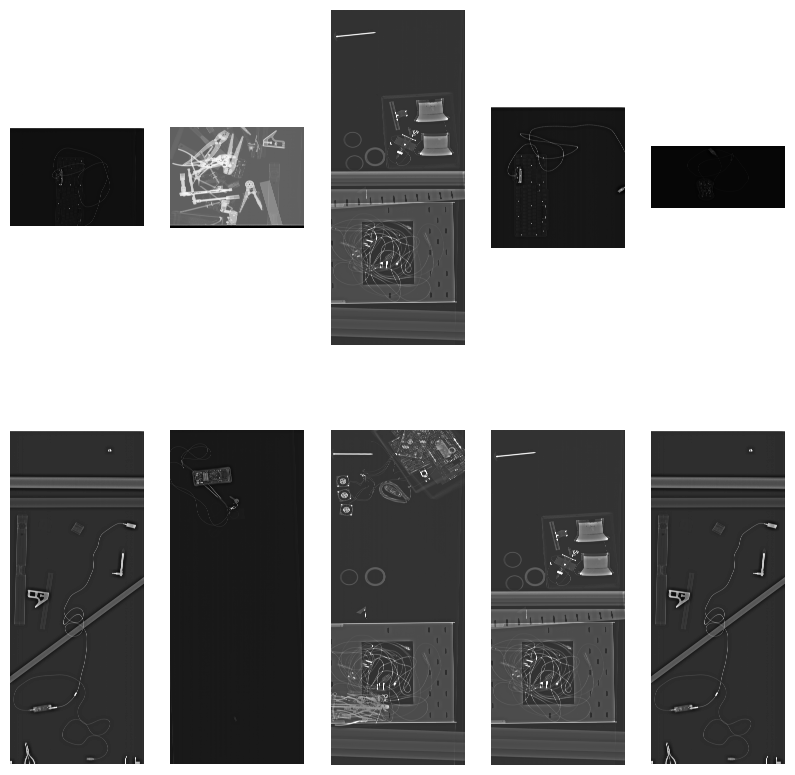
\includegraphics[width=0.7\linewidth]{3_Chapters//3_Chapter_Methodology//Figures/Training Images grid.png}
    \caption{Set of training images collected}
    \label{fig:trainingset}
\end{figure}

\section{Deep Learning Models}
The two models, \gls{N2N} and \gls{N2V} selected in section \ref{sec:modsec} above, are discussed below in terms of their theory and architecture. To understand these models effectively, a brief overview of traditional \gls{CNN}s is explored first to lay the groundwork required to understand the adaptions made to the \gls{N2N} and \gls{N2V} models.


\subsection{Traditional \gls{CNN}}
\textbf{Theory}\\
Traditional \gls{CNN}s learn to denoise images by mapping corrupted observations to clean versions.  This is done through training a \gls{CNN} with a large number of input and ground truth pairs($x_i,y_i$) and then minimising the empirical risk as shown in Equation \ref{eq:emprisk} below:

\begin{equation}
	\arg\min_{\theta} \sum_{i} L\left( f_{\theta}(\hat{x}_i), y_i \right)
	\label{eq:emprisk}
\end{equation}
Where:
\begin{table}[h!]
\begin{tabular}{ll}
	$f_{\theta}$ & represents a parametric family of mappings (e.g., \gls{CNN}s), under the loss function L.  \\
	$\hat{x}_i$ & shows the corrupted input $\hat{x}_i \sim p(\hat{x}_i | y_i)$  is a random variable distributed according to the clean target.\\
\end{tabular}
\end{table}

This can be broken down further by treating each pixel prediction in output to have a specific receptive field $x_{RF}(i)$, i.e the set of input pixels influencing that output pixel prediction. Consequently, this shows that denoising can be achieved by extracting overlapping patches and feeding them to the network one by one, rendering the parametric mapping from equation \ref{eq:emprisk}to be rewritten as:
\begin{equation}
	f({{\mathbf{x}}_{{\text{RF}}(i)}};\theta ) = {\hat y_i}
	\label{eq:parmap}
\end{equation}

The training inputs are now seen as pairs(${\mathbf{x}}_{{\text{RF}}(i)}^j$, ${\mathbf{y}}_i^j$) where ${\mathbf{x}}_{{\text{RF}}(i)}^j$ is a patch around pixel i, extracted from the training input image and ${\mathbf{y}}_i^j$ is the corresponding target pixel value, extracted from the ground truth image at the same position. This now leads to the Equation \ref{eq:emprisk} above to be refactored to Equation \ref{eq:empriskmod}:

\begin{equation}
	\mathop {\arg \min }\limits_\theta \sum\limits_j \sum\limits_i L\left( f({\mathbf{x}}_{{\text{RF}}(i)}^j;\theta ) = {\mathbf{\hat y}}_i^j, {\mathbf{y}}_i^j \right)
	\label{eq:empriskmod}
\end{equation}


With an \gls{MSE} Loss defined as:

\begin{equation}
	L\left( {\mathbf{\hat y}}_i^j, {\mathbf{y}}_i^j \right) = \left( {\mathbf{\hat y}}_i^j - {\mathbf{y}}_i^j \right)^2
	\label{eq:loss}
\end{equation}

\textbf{Architecture}\\
The \gls{CNN} architecture that is of interest in our study is the \gls{U-Net} architecture since both \gls{N2N} and \gls{N2V} modify this neural net type in their respective implementations. Additionally, it is widely used in medical image denoising because it can produce accurate segmentation even with small training datasets.  A typical U-net generally consists of two key parts:

\begin{enumerate}
	\item \textbf{Contracting path:} responsible for identifying relevant features in an image through using encoder layers to perform convolution operations to reduce the spatial resolution of feature maps whilst increasing their depth to capture abstract representations of the input. 
	\item \textbf{Expansive path:} Focuses on decoding the encoded data from the contracting path to locate the features whilst maintaining the input's spatial resolution. This is done through upsampling and performing convolutional operations.
\end{enumerate}

An example of \gls{U-Net} architecture is shown in Figure \ref{fig:Unet} below:
\begin{figure}[h!]
	\centering
	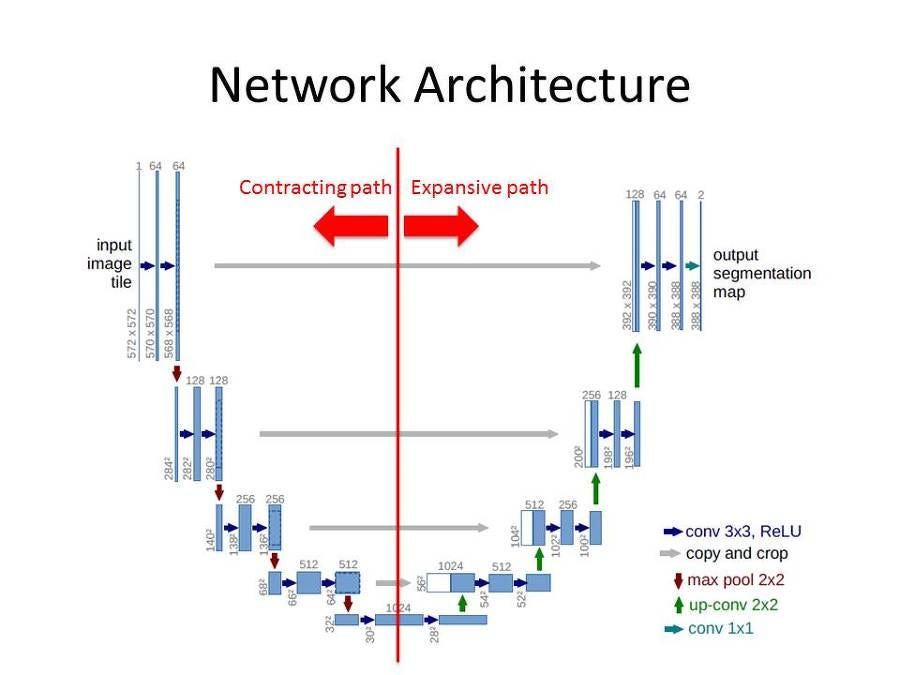
\includegraphics[width=0.7\linewidth]{3_Chapters//3_Chapter_Methodology//Figures/Unet.jpg}
	\caption{illustrates the \gls{U-Net} architecture, which transforms a grayscale input image into a smaller binary segmentation map using a contracting-expansive path with skip connections and no padding, progressively reducing spatial dimensions while increasing feature depth.}
	\label{fig:Unet}
\end{figure}


\subsection{\gls{N2N}}

\textbf{Theory}\\
N2N improves on the traditional CNN model by eliminating the dependency on input data on the equation \ref{eq:emprisk} and using a trivial $f_{\theta}$ that outputs a learned scalar. This task reduces to a loss function, which can be viewed as an \gls{ML} estimation by interpreting the loss function as the negative log-likelihood as shown in equation \ref{eq:min_expectation} below:
\begin{equation}
	\arg\min_{\theta} \mathbb{E}_{x} \left\{ \mathbb{E}_{y|x} \left[ L(f_{\theta}(x), y) \right] \right\}
	\label{eq:min_expectation}
\end{equation}
From the above, it is deduced that the network can solve the point estimation problem separately for each input sample. Thus \gls{N2N} works on the principle that the property of L2 minimisation that on expectation, the estimate remains unchanged when the targets are replaced with random numbers whose expectations match the targets. Consequently, the loss function holds under these conditions, and the optimal network parameters $\theta$ of Equation \ref{eq:min_expectation} also remain unchanged, if input-conditioned target distributions $p(y|x)$  are replaced with arbitrary distributions that have the same conditional expected values.  As a consequence and  factoring in the use of corrupted inputs the empirical minimisation task reduces to equation \ref{eq:min_loss} below:
\begin{equation}
	\arg\min_{\theta} \sum_{i} L\left( f_{\theta}(\hat{x}_i), \hat{y}_i \right)
	\label{eq:min_loss}
\end{equation}

With inputs being drawn from a corrupted distribution that is conditioned on the underlying, unobserved clean target $y_i$ such that  $E\{\hat{y}_i|\hat{x}_i\} = y_i$, given an infinite data, the solution is the same as that of equation \ref{eq:emprisk} of traditional \gls{CNN}.

\gls{N2N}  starts with  a pair of  noisy image pairs  ($x^j$, $x^{j'}$), where

\begin{equation}
	x^j = s^j + n^j \quad \text{and} \quad x^{j'} = s^{j'} + n^{j'}
	\label{eq:noisemodel}
\end{equation}

The two training images are identical up to their noise components $n^j, n^{j'}$. Applying patch-based approach the training data is then viewed as pairs ${\mathbf{x}}_{{\text{RF}}(i)}^j, {{\mathbf{x}}_i}^{'j}$, consisting of a noisy input patch ${\mathbf{x}}_{{\text{RF}}(i)}^j$, extracted from $x^j$, and a noisy target, taken from $x^{'j}$ at the position i. Similarly, to traditional \gls{CNN} training, parameters are tuned to minimise the loss in equation \ref{eq:loss}, however, the only difference is that a noisy target is being used instead of ground truth data $y_i$. 

\textbf{Architecture} \\
\gls{N2N} architecture is a modified \gls{U-Net} architecture consisting of the following three key parts:
\begin{enumerate}
	\item \textbf{Contraction Part:} The contraction part consists of multiple Conv2D layers with 3x3 filters, typically using 64 filters to capture features from the input image. Optional dropout layers can be included to prevent overfitting by randomly zeroing a fraction of input units during training. Max-pooling layers with 2x2 filters are used to down-sample the feature maps, reducing spatial dimensions while retaining important features.
	\item \textbf{Bottleneck Part:} In the bottleneck, two Conv2D layers with 3x3 filters further process the down-sampled feature maps. Optional dropout layers can be applied to prevent overfitting. Up-sampling with 2x2 layers increases the spatial dimensions, preparing the feature maps for the expansion phase.
	\item \textbf{Expansion Part:} The expansion part includes Conv2D layers with 3x3 filters to refine the up-sampled feature maps and reconstruct the denoised image. Optional dropout layers help improve generalisation. 2x2 up-sampling layers restore the spatial dimensions of the feature maps to match the original input size.
\end{enumerate}
The architecture of a sample \gls{N2N} is visualised in Figure \ref{fig:N2Narch} below:

\begin{figure}[h!]
	\centering
	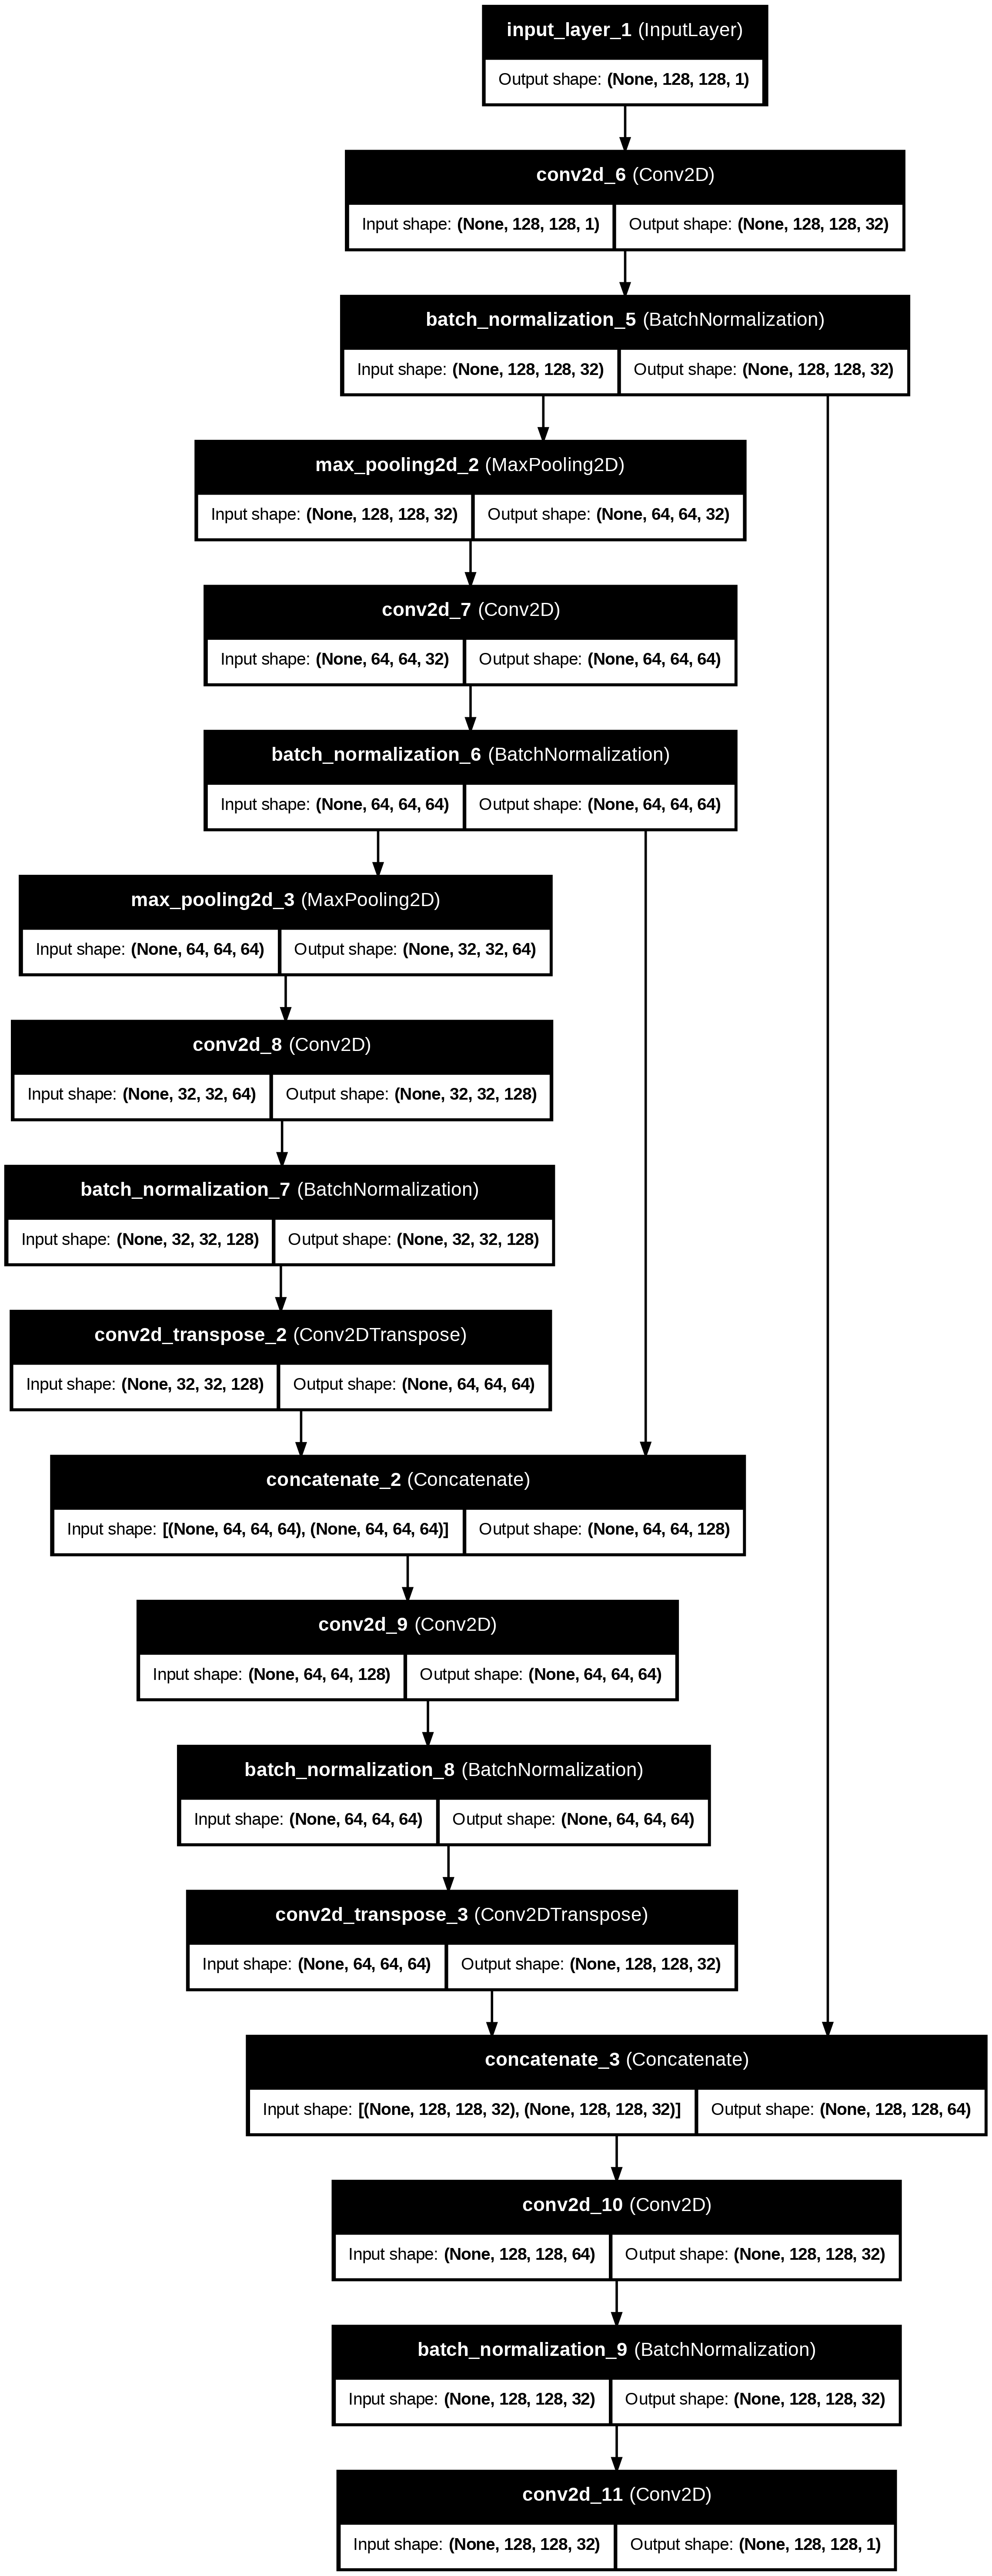
\includegraphics[width=0.5\linewidth]{3_Chapters//3_Chapter_Methodology//Figures/noise2noise_model.png}
	\caption{\gls{N2N} architecture}
	\label{fig:N2Narch}
\end{figure}


\subsection{\gls{N2V}}
\textbf{Theory} \\
\gls{N2V} is an extension of \gls{N2N} in that it proposes that the two patches be extracted from a single image instead of two.  It is based on the principle that upon extraction of a patch, the centre pixel can be masked and used as the target, allowing the network to learn to map the value at the centre of the input patch directly to the output. 

To achieve this \gls{N2V} has a set of assumptions:

\begin{enumerate}
	\item Image generation is seen as ${\mathbf{x}} = {\mathbf{s}}+ {\mathbf{n}}$ as a draw from the joint distribution $p({\mathbf{s}},{\mathbf{n}}) = p({\mathbf{s}})p({\mathbf{n}}|{\mathbf{s}})$
	\item $p({\mathbf{s}})$ is assumed to be an arbitrary distribution satisfying $p({{\mathbf{s}}_i}|{{\mathbf{s}}_j}) \ne p({{\mathbf{s}}_i})$ for two pixels i and j within a certain radius of each other, with pixel ${{\mathbf{s}}_i}$ of the signal not statistically independent. \label{it:second}
	\item With respect to ${\mathbf{n}}$ a conditional distribution of the following form is assumed: $p({\mathbf{n}}|{\mathbf{s}}) = \prod\limits_i {p({{\mathbf{n}}_i}{{\mathbf{s}}_i})} $, indicating pixels values of the noise are conditionally independent given the signal.
	\item Noise is assumed to be zero-mean i.e $\mathbb{E}[{{\mathbf{n}}_i}] = 0$ leading to $\mathbb{E}[{{\mathbf{x}}_i}] = {{\mathbf{s}}_i}$ \label{it:fourth}
\end{enumerate}

Based on the above assumptions, it can be deduced that acquiring multiple images with the same underlying signal but different noise realisations, and then averaging them, will converge toward the true signal.

\gls{N2V} uses a special receptive field with a blind spot at its centre, as shown in Figure \ref{fig:blind} below; thus, \gls{CNN} prediction ${{\mathbf{\hat s}}_i}$ for a pixel is affected by all input pixels in a square neighbourhood except for the input pixel ${{\mathbf{x}}_i}$ at its very location. This leads to less information than a traditional \gls{CNN}; however, this is the advantage of the blindspot network i.e. its inability to learn identities. This is done by a masking scheme that replaces the value in the centre of each input patch with a randomly selected value from the surrounding area.

\begin{figure}[h!]
	\centering
	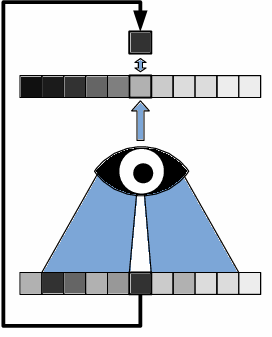
\includegraphics[width=0.3\linewidth]{3_Chapters//3_Chapter_Methodology//Figures/blindspot.png}
	\caption{Blind-spot network showing the receptive field of a pixel, excluding the pixel itself.}
	\label{fig:blind}
\end{figure}

The noise is assumed to be pixel-wise independent; thus, neighbouring pixels carry no information about the pixel, and therefore, it is impossible to produce an estimate that is better than a priori expected value(see \ref{it:fourth}). However, this is countered by the signal being assumed to contain statistical dependencies (see \ref{it:second}). As a result, the network can still estimate the signal ${{\mathbf{s}}_i}$ of a pixel by looking at its surroundings.  Consequently, the blind network allows extraction of input patch and target value from the same noisy image. Thus the empirical risk becomes:

\begin{equation}
	\mathop {\arg \min }\limits_\theta \sum\limits_j {\sum\limits_i {L\left( {f({\mathbf{\tilde x}}_{{\text{RF}}(i)}^j;\theta ),{\mathbf{x}}_i^j} \right)} } 
	 \label{eq:minn2v}
\end{equation}

The target ${\mathbf{x}}_i^j$ is equivalent to \gls{N2N}'s ${\mathbf{x}}_i^{‘j}$ which is extracted from the second image. The two target values ${\mathbf{x}}_i^j$ and ${{\mathbf{x}}_i^{‘j}}$ have an equal signal ${{\mathbf{s}}_i^j}$with noise components being two independent samples from the same distribution $p({{\mathbf{n}}_i}|{{\mathbf{s}}_j})$. This, in principle, shows that using a blindspot network, an individual noisy image can be used to train the model. 

\textbf{Architecture}\\
\gls{N2V} is  based on a modified \gls{U-Net} architecture and consists of three main sections:

\begin{enumerate}
	\item \textbf{Contraction Part}: Multiple Conv2D layers with 3x3 filters (typically 64 filters each) capture features from the input image. Optional dropout layers prevent overfitting, and 2x2 max-pooling layers down-sample the feature maps, reducing spatial dimensions while retaining important features.
	\item \textbf{Bottleneck Part}: Two Conv2D layers with 3x3 filters further process the down-sampled feature maps. Optional dropout layers are included, and 2x2 up-sampling layers increase the spatial dimensions of the feature maps, preparing them for the expansion part.
	\item \textbf{Expansion Part}: Multiple Conv2D layers with 3x3 filters refine the up-sampled feature maps and reconstruct the denoised image. Optional dropout layers enhance generalisation, and 2x2 up-sampling layers restore the feature maps to the original input size. 
\end{enumerate}
A visual representation of the architecture is shown in Figure \ref{fig:N2Varch} below:
\begin{figure}[h!]
	\centering
	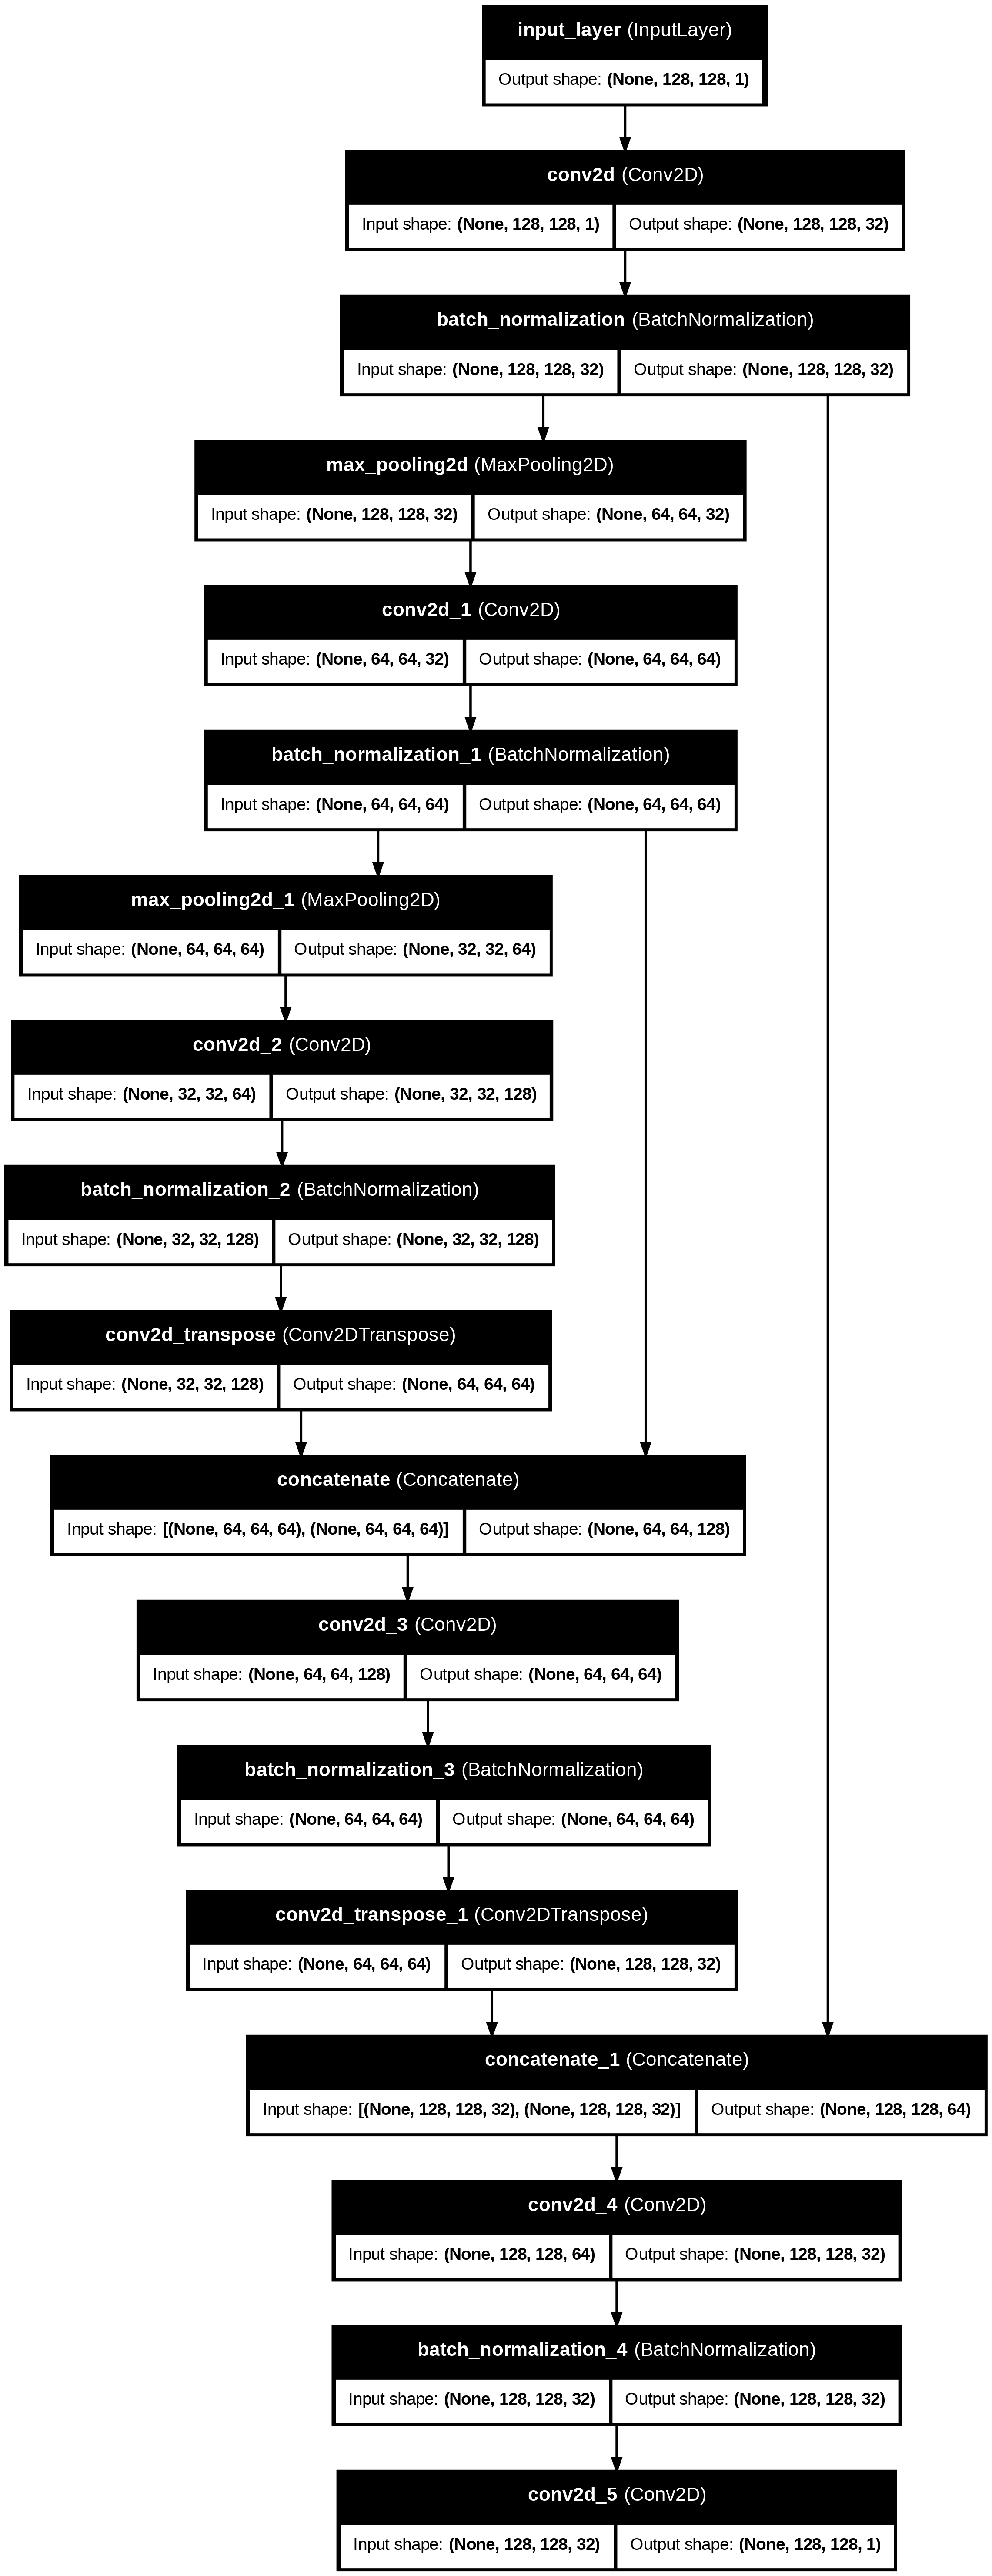
\includegraphics[width=0.5\linewidth]{3_Chapters//3_Chapter_Methodology//Figures/noise2void_model.png}
	\caption{\gls{N2V} architecture}
	\label{fig:N2Varch}
\end{figure}

\section{Research Instruments}
\subsection{Software}
The software was crucial for two parts of the process. First, software was needed to interface with the LODOX\textsuperscript{\textregistered} Statscan\textsuperscript{\textregistered} scanner to collect data. The software used to interface with the scanner was the DVS\textsuperscript{\textregistered} by LODOX\textsuperscript{\textregistered} Systems Pty Limited. It was also used to get the raw image and export it into \gls{DICOM} file format for denoising in other software platforms. 

Secondly, software was needed to develop the denoising model.The choice of programming language to develop the denoising model is critical to ensure the model is effectively implemented, scalable, and maintainable while providing access to necessary libraries and tools for medical image processing. Per the user requirements outlined in section \ref{sec:reqs} above, the following programming languages were considered: Python and MATLAB\textsuperscript{\textregistered}. The criteria for choosing a programming language for implementation were : 

\begin{itemize}
	\item Ease of development
	\item Community support
	\item Integration with deep learning frameworks
	\item \gls{DICOM} Support
	\item Integration and Interoperability
\end{itemize}

A detailed comparison is shown in Table \ref{tab:progcomp} below:

\begin{table}[h!]
	\centering
	\caption{Comparison of Python and MATLAB\textsuperscript{\textregistered}}
	\label{tab:progcomp}
	\begin{tabular}{@{}p{2.9cm}p{5cm}p{5cm}@{}}
		\toprule
		\textbf{Criteria} &
		\textbf{Python} &
		\textbf{MATLAB\textsuperscript{\textregistered}} \\ \midrule
		Deep Learning Frameworks &
		Extensive library support for deep learning (TensorFlow, PyTorch, Keras) &
		Built-in tools for image processing and analysis (Deep Learning Toolbox, Image Processing Toolbox). \\
		\gls{DICOM} Support &
		Strong support for medical imaging (pydicom, SimpleITK) &
		Robust support for \gls{DICOM} and medical image processing. \\
		Community support &
		A large, active community with vast resources makes finding help and solutions easier. &
		Strong academic support but a smaller community compared to Python for deep learning. \\
		Ease of development &
		Fast prototyping with a vast array of pre-built models and functions available. &
		Very efficient for initial development and testing with built-in functions for common tasks. \\
		Integration and Interoperability &
		Integrates well with other software and tools, making it highly flexible. &
		Excellent integration with hardware and other MathWorks products.
	\end{tabular}
\end{table}

Python is chosen as the primary programming language for implementing the two denoising model due to its extensive library support, ease of use, and strong community resources as depicted in Table \ref{tab:progcomp} above. 


\subsection{Hardware}
The LODOX\textsuperscript{\textregistered} Statscan\textsuperscript{\textregistered} scanner model was used to do the scans. It is housed at the Medical Imaging Lab, UCT HUB, Division of Biomedical Engineering. The other hardware used were the phantoms that were being scanned to provide images for model training, validation and testing as was detailed in section \ref{sec:datacolelction}. 



\section{Performance metrics}
The following groups of performance metrics were used to measure the performance metrics: Proxy quantitative, qualitative, and no-reference quality and are discussed in detail below:


\subsection{Proxy Quantitative Analysis}
Traditional metrics like \gls{SNR}, \gls{PSNR} and \gls{SSIM} cannot be used directly as there is no access to clean images; thus, proxy versions of these metrics were used by treating the denoised image as a proxy for the clean image and comparing it with the original noisy input. This will give relative noise performance. These proxy measurements are discussed in Table \ref{tab:metrics} below:

\begin{table}[h!]
	\centering
	\caption{Proxy Quantitative Analysis}
	\label{tab:metrics}
	\begin{tabular}{@{}lp{10cm}@{}}
		\toprule
		\textbf{Metric}         & \textbf{Importance}                                                                                                              \\ \midrule
		pseudo-\gls{SNR}              & Quantifies the noise level relative to image signal with higher \gls{SNR} values indicating beer noise suppression                     \\
		pseudo-\gls{PSNR}             & Measures the peak error between the original and denoised images, with higher values indicating better performance.              \\
		pseudo-\gls{SSIM} &
		Evaluates the similarity between the original and denoised images based on luminance, contrast, and structure. It is vital to ensure that the structural integrity of  LODOX\textsuperscript{\textregistered} Statscan\textsuperscript{\textregistered} images is maintained. \\
		Noise Residual Analysis & Analyses the difference between the noisy input and denoised output to assess the efficacy of the model in denoising the image. \\ \bottomrule
	\end{tabular}
\end{table}

\subsection{Qualitative Metrics}
Drawing from \cite{juneja_denoising_2024} quality analysis, the denoised images were visually compared against the processed output from the DVS\textsuperscript{\textregistered} software using an eye test to assess image quality. Additionally, the denoised images were compared to their noisy counterparts to evaluate differences in clarity, contrast, and overall usability. This visual assessment helps to identify improvements in image quality and ensures that the denoising process enhances the diagnostic value of the images without introducing artifacts or losing critical information.


\subsection{No-Reference Quality Metrics}
The following no-reference metrics were used to evaluate the image quality since they were inherently

designed to assess image quality without needing a clean reference image. The following no-reference metrics were used:

\begin{itemize}
	\item \gls{NIQE}: This model evaluates image quality by measuring deviations from statistical regularities found in natural images.
	\item \gls{BRISQUE}: calculates quality using features that capture natural scene statistics.
	\item \gls{PIQE}: computes image quality based on perceptual information in localised spatial regions of the image.
\end{itemize}

\section{Limitations}
\begin{enumerate}
	\item \textbf{Use of Non-Anatomical Phantoms}: The study utilizes non-clinical phantoms that do not accurately model human tissue. This limitation may hinder the direct application of findings to clinical settings, as the phantoms lack the anatomical complexities present in actual human subjects, potentially impacting the generalisability of the results.
	\item \textbf{Time Constraints on Model Training}: The machine learning models were trained within the confines of a 12-week project duration. Extended training time could have improved the efficacy and performance of these models. The limited training period may not have allowed the models to be fully optimised, potentially affecting the robustness of the denoising outcomes.
	\item \textbf{Limited Scope of Unsupervised Models}: The methodology considers only two unsupervised denoising models. While there is potential for better performance with additional models, the study is constrained by the availability and maturity of unsupervised techniques. As discussed in Chapter 2, most advanced denoising models currently rely on supervised learning, which limits the exploration of a broader range of unsupervised approaches.
\end{enumerate}
These limitations highlight areas where the methodology could be refined in future studies, such as the inclusion of more realistic phantoms, extended training periods, and the exploration of a wider variety of unsupervised denoising models.


\section{Ethics}
Ethics was complied with as set out and specified by the UCT Ethics guideline and guidelines stipulated by the EBE faculty. No human subjects are used in the research, and the use of Artificial Intelligence in this research qualifies as minimal risk. A detailed Ethics approval and application form is detailed in Appendix B. 



\section{Conclusion}
In conclusion, this chapter provided a comprehensive overview of the research methodology employed in developing the denoising model for LODOX\textsuperscript{\textregistered} Statscan\textsuperscript{\textregistered}images. The research design was carefully structured, beginning with exploring relevant literature and progressing through preliminary data collection, model selection, and the rigorous testing and validation of the chosen models. The methodology emphasised the importance of selecting appropriate phantoms and utilising both classical and advanced deep learning techniques to achieve the desired denoising outcomes. The software and hardware tools were carefully chosen to ensure compatibility and efficiency, with Python emerging as the preferred language due to its extensive library support and scalability in machine learning tasks.

The analysis phase utilised a combination of quantitative metrics, such as \gls{SNR}, \gls{PSNR}, and \gls{SSIM}, alongside qualitative assessments to validate the effectiveness of the denoising models. Despite the limitations of using non-anatomical phantoms and the constrained training period, the study successfully demonstrated the potential of unsupervised deep learning models, particularly \gls{N2N} and \gls{N2V}, in enhancing the quality of LODOX\textsuperscript{\textregistered} Statscan\textsuperscript{\textregistered}images. 

